\usepackage{comment}

\newcommand{\tblParamTradeoffs}{
  \begin{table}[h]
    \begin{center}
      \caption{Trade-offs between FHE parameters.}
      \begin{footnotesize}
        \begin{tabular}{ c | c c }
          \toprule
          & Small $N$ & Big $N$ \\
          \midrule
          Big $Q$ & Not secure & Sweet spot \\
          Small $Q$ &  \multicolumn{2}{c}{Cannot bootstrap} \\
          \bottomrule
        \end{tabular}
      \end{footnotesize}
    \end{center}
    \label{tbl:paramTradeoffs}
  \end{table}
}

\newcommand{\figParamTradeoffs}{
  \begin{figure}[h]
        \begin{center}
     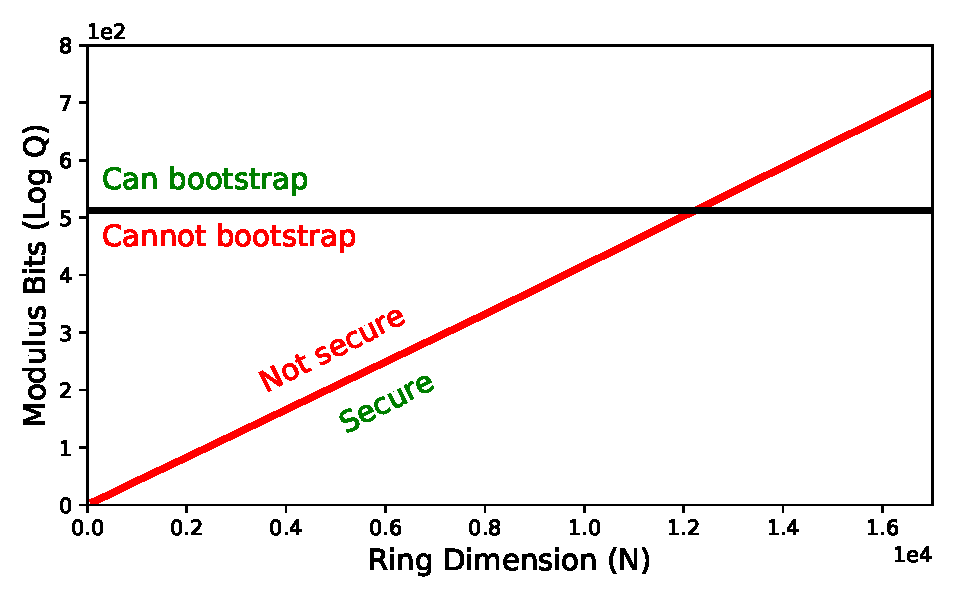
\includegraphics[width=0.75\columnwidth]{plots/security.pdf}
    \caption{Trade-offs between FHE parameters. Parameter values above the
      red line are deemed insecure (i.e., correspond to a security parameter below $80$ bits). The
      parameter values below the black line do not allow for bootstrapping.}
    \label{fig:paramTradeoffs}
    \vspace{-0.03in}
    \end{center}
  \end{figure}
}

\newcommand{\figArch}{
  \begin{figure}[h]
        \begin{center}
     \includegraphics[width=\columnwidth]{figures/ag_arch.pdf}
     \vspace{-0.12in} % this negative vspace... adds space  (which is what I want)
     \caption{Overview of the \name architecture.}
     \vspace{0.025in} % leave bottoms flush
    \label{fig:arch}
  \end{center}
  \end{figure}
}

\newcommand{\figMultDataflow}{
  \begin{figure}[h]
        \begin{center}
     \includegraphics[width=0.99\columnwidth]{figures/ag_mult_dataflow.pdf}
    \caption{Example matrix-vector multiply using FHE.}
    \label{fig:MultDataflow}
    \vspace{-0.1in}
    \end{center}
  \end{figure}
}

\newcommand{\figOpBreakdown}{
    \begin{figure}[h]
    \begin{center}
        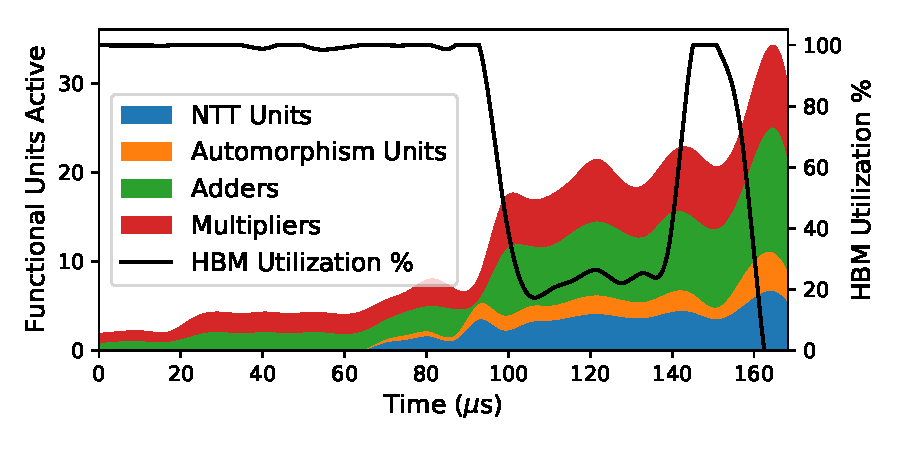
\includegraphics[width=0.7\columnwidth]{plots/lolaptwTimeplot.pdf}
        \caption{Functional unit and HBM utilization over time for the LoLa-MNIST PTW benchmark.}
        \label{fig:opBreakdown}
    \end{center}
    \end{figure}
}

\newcommand{\figCompilerOverview}{
  \begin{figure}[h]
        \begin{center}
     \includegraphics[width=\columnwidth]{figures/ag_compiler_overview.pdf}
    \caption{Overview of the \name compiler.}
    \label{fig:compilerOverview}
    %\vspace{-0.06in} %dsm: Shaves off a line, but looks bad
    \end{center}
  \end{figure}
}

\newcommand{\figautfu}{
\setlength{\columnsep}{7pt}
  \begin{figure}[h]
    \begin{center}
      \vspace{-0.8em}
     \includegraphics[width=0.25\columnwidth]{figures/ag_aut_fu.pdf}
    \caption{Automorphism unit.}
    \label{fig:aut_fu}
    \vspace{-0.4em} 
    \end{center}
  \end{figure}
}

\newcommand{\figAutomorphism}{
  \begin{figure}[h]
        \begin{center}
    \includegraphics[width=0.99\columnwidth]{figures/ag_automorphism.pdf}
    \caption{Applying $\sigma_3$ on a ciphertext of four 4-element chunks by using only permutations local to chunks.}
    \label{fig:automorphism}
    \end{center}
  \end{figure}
}

\newcommand{\figTranspose}{
  \begin{figure}[h]
    \centering
    \includegraphics[width=0.5\columnwidth]{figures/ag_transpose.pdf}
    \caption{The transpose unit.}
    \label{fig:transpose}
  \end{figure}
}

\newcommand{\figFourStepNTT}{
  \begin{figure}[h]
    \includegraphics[width=0.99\columnwidth]{figures/ag_four_step_ntt.pdf}
    \caption{Example of a four-step NTT datapath that uses 4-point NTTs to implement 16-point NTTs.}
    \label{fig:fourStepNTT}
    \vspace{1em}
  \end{figure}
}

\newcommand{\figQuadrantSwap}{
  \begin{figure}[h]
    \centering
    \includegraphics[width=0.75\columnwidth]{figures/ag_quadrant_swap.pdf}
    \caption{Transpose unit (right) and its component quadrant-swap unit (left).}
    \label{fig:quadrantSwap}
    \vspace{0.1in}
  \end{figure}
}

\newcommand{\figOverview}{
  \begin{figure}[h]
    \centering
    \vspace{-0.11in}
    \includegraphics[width=.8\columnwidth]{figures/ag_overview.pdf}
    \caption{FHE allows a user to securely offload computation to an untrusted server.}
    %old: \caption{Workflow showing how FHE is used to securely offload computation to an untrusted server.}
    \label{fig:overview}
    \vspace{0.2cm}
  \end{figure}
}

\newcommand{\figFUSweep}{
  \begin{figure}[h]
        \begin{center}
     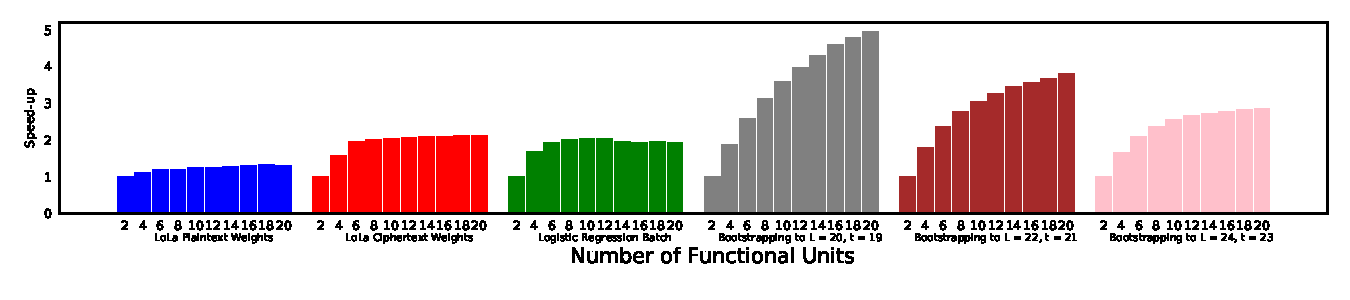
\includegraphics[width=\columnwidth]{plots/sweepFUs.pdf}
    \caption{Performance of our benchmarks with varying number of functional unit clusters.}
    \label{fig:sweepFUs}
    \vspace{-0.03in}
    \end{center}
  \end{figure}
}

\newcommand{\figBWSweep}{
  \begin{figure}[h]
        \begin{center}
     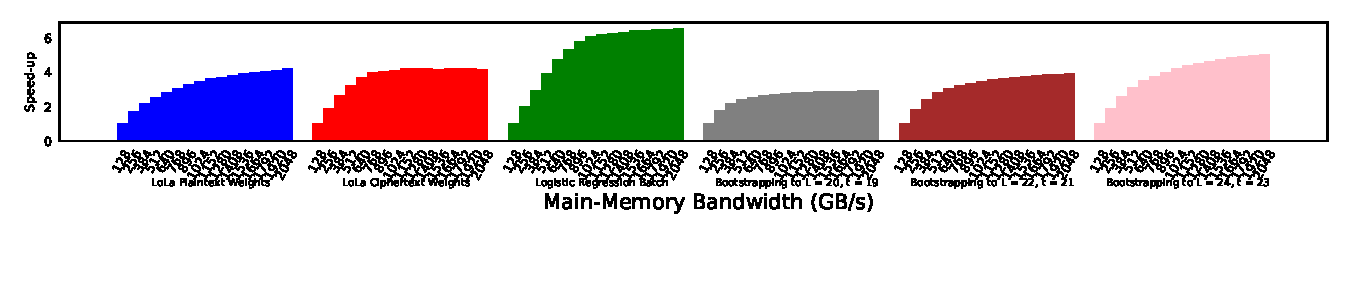
\includegraphics[width=\columnwidth]{plots/sweepBW.pdf}
    \caption{Performance of our benchmarks across various main memory bandwidths.}
    \label{fig:sweepBW}
    \vspace{-0.03in}
    \end{center}
  \end{figure}
}

\newcommand{\figDataMovement}{
\begin{figure}
  \centering
  \subfloat[]{
    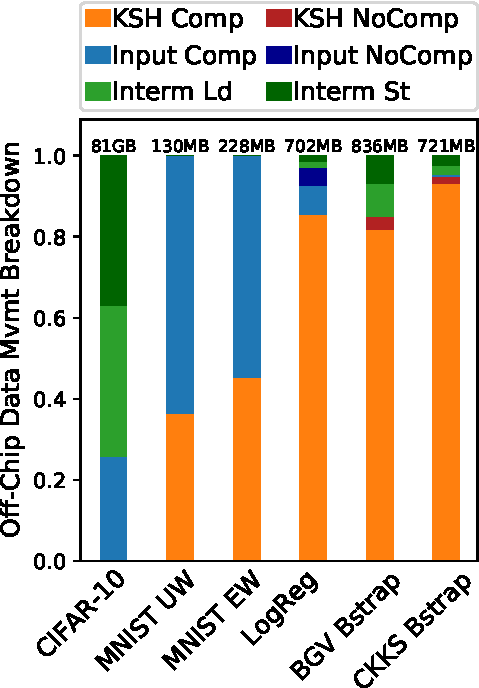
\includegraphics[width=0.4\linewidth]{plots/dataMovement.pdf}
    \label{fig:dataMovement}
  }
  \subfloat[]{
    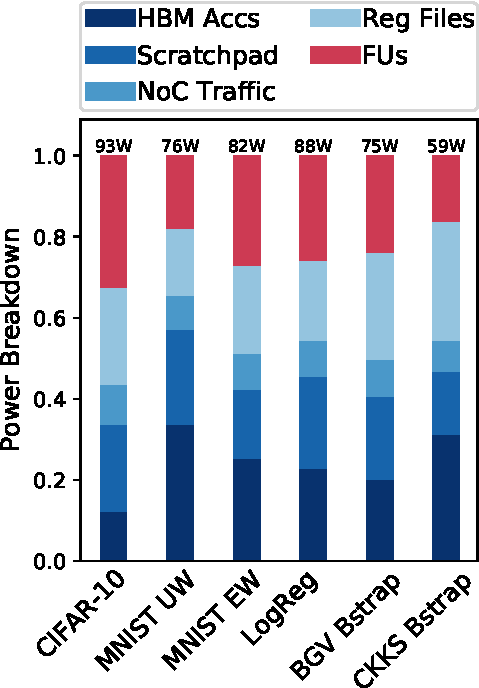
\includegraphics[width=0.4\linewidth]{plots/power.pdf}
    \label{fig:power}
  }
  \caption{Per-benchmark breakdowns of \textbf{(a)} data movement and \textbf{(b)} average power for \name.}
  %\vspace{0.1in}
\end{figure}
}

\newcommand{\figConfigs}{
    % \setlength{\columnsep}{7pt}
  \begin{figure}[h]
    % \vspace{-0.55in}
    \begin{center}
     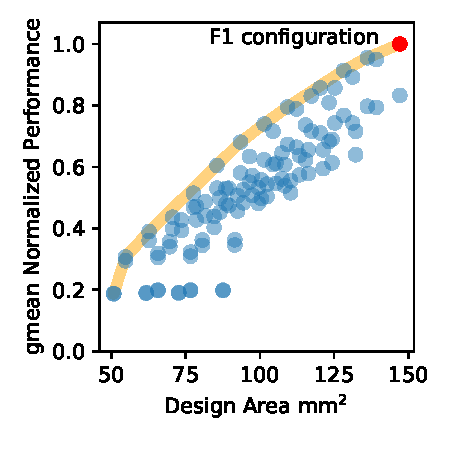
\includegraphics[width=0.45\columnwidth]{plots/configs.pdf}
    % \vspace{-0.26in}
    \caption{Performance vs. area across \name configurations.}
    \label{fig:pareto}
    % \vspace{-18pt}
    % \hspace{-0.03in}
    \end{center}
  \end{figure}
}

\newcommand{\figScratchpadSweep}{
  \begin{figure}[h]
        \begin{center}
     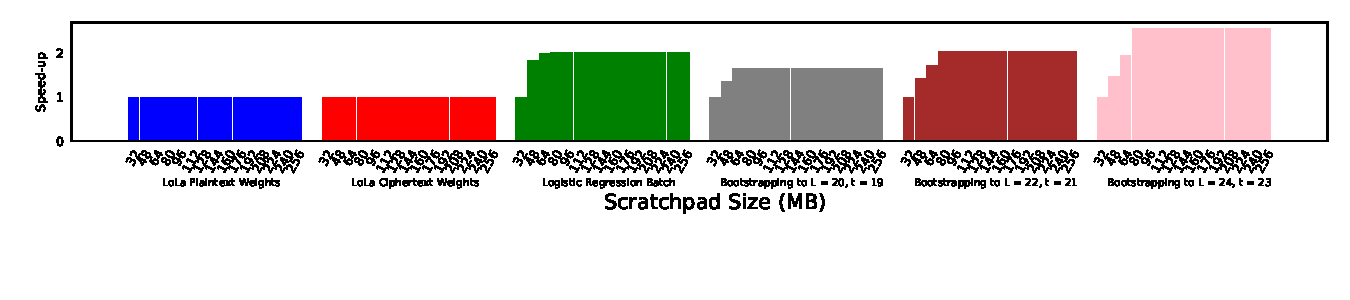
\includegraphics[width=\columnwidth]{plots/sweepScratchpad.pdf}
    \caption{Performance of our benchmarks across various scratchpad sizes.}
    \label{fig:sweepScratchpad}
    \vspace{-0.03in}
    \end{center}
  \end{figure}
}

\newcommand{\tblGF}{
  \begin{table}[h]
    \begin{center}
      \begin{footnotesize}
        \begin{tabular}{lrrr}
          \toprule
          Component & Area [mm$^2$] & TDP [W] \\
          \midrule
          NTT FU & 2.27 & 4.80  \\
          Automorphism FU & 0.58 & 0.99  \\
          %Transpose & 0.28 & \tmp{???} & - \\
          Multiply FU & 0.25 & 0.60  \\
          Add FU & 0.03 & 0.05  \\
          Vector RegFile (512\,KB) & 0.56 & 1.67 \\
          \textbf{Compute cluster} & 3.97 & 8.75 \\
          (NTT, Aut, 2$\times$ Mul, 2$\times$ Add, RF) & & \\
          \textbf{Total compute} (16 clusters) &  \textbf{63.52} & \textbf{140} \\
          \midrule
          Scratchpad (16$\times$4\,MB banks) & 48.09 & 20.35 \\
          3$\times$NoC (16$\times$16 512\,B bit-sliced~\cite{passas:tocaid12:crossbar}) & 10.02 & 19.65 \\
          Memory interface (2$\times$HBM2 PHYs) & 29.8 & 0.45 \\
          \textbf{Total memory system} &  \textbf{87.91} & \textbf{40.45} \\
          \midrule
          \textbf{Total \name} &  \textbf{151.43} & \textbf{180.45} \\
          \bottomrule
        \end{tabular}
      \end{footnotesize}
    \end{center}
    \vspace{-0.08in}
    \caption{Area and Thermal Design Power (TDP) of \name, and breakdown by component.}
    \label{tbl:GF12}
    \vspace{-0.1in}
  \end{table}
}


\newcommand{\tblNomenclature}{
   \begin{table}[h]
     \begin{footnotesize}
        \begin{center}
           \begin{tabular}{ll}
              \toprule
              \textbf{Param} & \textbf{Definition} \\
              \midrule
               \multicolumn{2}{c}{FHE Parameters} \\
              \midrule
              $N$ & Number of vector elements / polynomial coefficients \\
              $Q$ & Ciphertext modulus \\
              $t$ & Plaintext modulus \\
              \midrule
               \multicolumn{2}{c}{Architecture Parameters} \\
              \midrule
              $L$ & Number of RNS polynomials per ciphertext polynomial \\
              $q_i$ & The $i$-th RNS modulus ($Q = q_0q_1...q_{L-1}$) \\
              $E$ & Number of vector lanes \\
              $V$ & Vector operation initiation interval ($V = N/E$) \\ % dsm: Chimes? I don't know of a good nomenclature for this...
              \bottomrule
           \end{tabular}
           \label{tbl:nomenclature}
        \end{center}
        \caption{Nomenclature of key parameters in this paper.}
     \end{footnotesize}
   \end{table}
}

\newcommand{\tblModMult}{
  \begin{table}[h]
    \begin{footnotesize}
      \begin{center}
        \begin{tabular}{lrrr}
          \toprule
          Multiplier & Area [$\mu$m$^2$] & Power [mW] & Delay [ps] \\
          \midrule
          Barrett & $5,271$ & $18.4$ & 1,317 \\
          Montgomery & $2,916$ & $9.2$ & 1,040 \\
          NTT-friendly & $2,165$ & $5.36$ & 1,000 \\ % assumes q = 2^11m+1
          \midrule
          \textbf{FHE-friendly (ours)} & $1,817$ & $4.1$ & 1,000 \\
          \bottomrule
        \end{tabular}
        \vspace{0.02in}
        \caption{Area, power, and delay of modular multipliers.}
        \label{tbl:modMult}
      \end{center}
    \end{footnotesize}
    \vspace{-0.18in}
  \end{table}
}

\newcommand{\x}{$\times$}


\newcommand{\tblMicrobenchmark}{
  \begin{table}[t]
      % \vspace{-0pt}
      \begin{center}
      \resizebox{\columnwidth}{!}{%
      \begin{tabular}{l|rrr|rrr|rrr}
        \toprule
        & \multicolumn{3}{c|}{$N = 2^{12}$, $\log Q = 109$} &
        \multicolumn{3}{c|}{$N = 2^{13}$, $\log Q = 218$} &
        \multicolumn{3}{c}{$N = 2^{14}$, $\log Q = 438$} \\
        
        & \textbf{\name} & vs.\ CPU & vs.\ HEAX$_\sigma$ & \textbf{\name} & vs.\ CPU & vs.\ HEAX$_\sigma$ & \textbf{\name} & vs.\ CPU & vs.\ HEAX$_\sigma$\\

        \midrule

        % --- NTT

        % N=2**12, logQ = 109
        NTT
        &\textbf{12.8} % our
        &17,148$\times$ % CPU
        &1,600$\times$ % HEAX

        % N=2**13, logQ = 218
        &\textbf{44.8} % our
        &10,736$\times$ % CPU
        &1,733$\times$ % HEAX

        % N=2**14, logQ = 438
        &\textbf{179.2} % our
        &8,838$\times$ % CPU
        &1,866$\times$ % HEAX
        \\
        % --- Automorph. w/out k-s
        
        % N=2**12, logQ = 109
        Automorphism 
        &\textbf{12.8} % our
        &7,364$\times$ % CPU
        &440$\times$ % HEAX

        % N=2**13, logQ = 218   
        &\textbf{44.8} % our
        &8,250$\times$ % CPU
        &426$\times$ % HEAX

        % N=2**14, logQ = 438
        &\textbf{179.2} % our
        &16,957$\times$ % CPU
        &430$\times$ % HEAX
        \\

        \midrule

        % --- Ctxt-Ctxt Mult.

        % N=2**12, logQ = 109    
        Homomorphic multiply
        &\textbf{60} % our - % 60 MULS * 32 * 1/(32) = 60 cycles
        &48,640$\times$ % CPU
        &172$\times$ % HEAX

        % N=2**13, logQ = 218
        &\textbf{300} % our
        &27,069$\times$ % CPU
        &148$\times$ % HEAX

        % N=2**14, logQ = 438
        &\textbf{2,000} % our
        &14,396$\times$ % CPU
        &190$\times$ % HEAX
        \\

        % --- Automorph. w/ k-s

        % N=2**12, logQ = 109    
        Homomorphic permutation
        &\textbf{40} % our
        &17,488$\times$ % CPU
        &256$\times$ % HEAX

        % N=2**13, logQ = 218
        &\textbf{224} % our
        &10,814$\times$ % CPU
        &198$\times$ % HEAX

        % N=2**14, logQ = 438
        &\textbf{1,680} % our
        &6,421$\times$ % CPU
        &227$\times$ % HEAX
        \\
        
        \bottomrule
      \end{tabular}
      }
      %}
      \end{center}
      %\vspace{-5pt}
      \caption{Performance on microbenchmarks: \name's \textbf{reciprocal throughput, in nanoseconds per ciphertext operation} (lower is better) and speedups over CPU and HEAX$_\sigma$ (HEAX augmented with scalar automorphism units) (higher is better).}
      \label{tbl:microbenchmark}
      %\vspace{-3pt} % dsm: Leaves flush with other pages
  \end{table}
    % dsm: Now explained in text
    %\footnotetext[2]{We assume an SRAM array is used to perform an automorphism via random reads because HEAX does not report how they implement automorphisms.}
    %     \footnotetext[3]{We assume throughput is bottleneck on either the automorphism or keyswitching throughput, whichever is smaller.}
}


\newcommand{\tblBenchmark}{
  \begin{table}[t]
    \begin{footnotesize}
      \begin{center}
      \begin{tabular}{lrrr}
        \toprule
        Execution time (ms) on & CPU & \name & Speedup \\
        
        \midrule
        LoLa-CIFAR Unencryp. Wghts. & $1.2\times10^6$ & \textbf{241} & $5,011$\x \\
        LoLa-MNIST Unencryp. Wghts. & $2,960$ & \textbf{0.17} & $17,412$\x \\
        LoLa-MNIST Encryp. Wghts. & $5,431$ & \textbf{0.36} & $15,086$\x \\
        Logistic Regression & $8,300$ & \textbf{1.15} & $7,217$\x \\
        BGV Bootstrapping & ---\footnotemark[2] & \textbf{1.8} & ---\footnotemark[2] \\  % L=24
        CKKS Bootstrapping & $1,554$ & \textbf{1.3} & $1,195$\x \\    % L=24
        \midrule

        \textbf{gmean speedup} &&& 6,471\x \\
        % CKKS Bootstrapping $L=22$ & $1456$ & \textbf{2.2} & $662$\x \\
        % CKKS Bootstrapping $L=20$ & $1314$ & \textbf{1.9} & $692$\x \\
        \bottomrule
      \end{tabular}
   \end{center}
    \vspace{-8pt}
      \hfill\footnotemark[1]{LoLa's release did not include MNIST with encrypted weights, so we reimplemented it in HELib.}\quad\mbox{} \\
      \hfill\footnotemark[2]{BGV bootstrapping in HELib crashes for this input, and we could not find an alternative implementation or fix HELib. We expect \name's speedup to be at least 3,000$\times$}.\quad\mbox{}
    \end{footnotesize}
    \vspace{4pt}
      \caption{Performance of \name and CPU on full FHE benchmarks: execution times in milliseconds
      and \name's speedup.}      
      \label{tbl:benchmark}
      \vspace{-6pt}
  \end{table}
}

\newcommand{\tblPrimitiveOps}{
  \begin{table}[h]
    \begin{footnotesize}
      \begin{center}
        \caption{Operations in BGV \cite{}, CKKS \cite{}, and GSW \cite{} schemes and their constituent
        \textit{primitive operations}, which \name FUs acelerate. BGV and CKKS use very similar FHE operations
        and differ mainly in encryption/decryption.}
        \begin{tabular}{l|rr}
          \toprule
          & \multicolumn{2}{c}{\textbf{Required primitive operations}} \\
          \textbf{Operation} & \textbf{BGV/CKKS} & \textbf{GSW} \\
          \midrule
          Ciphertext add & add & add \\
          Ciphertext mult & NTT, mult & NTT, mult, add \\
          Key switching/relin & NTT, mult, add & N/A \\
          Mod switching & NTT, reduce, add & NTT, reduce, add \\
          Bootstrapping & automorphism, all ops & automorphism, all ops \\
          \bottomrule
        \end{tabular}
        \label{tbl:primitiveOps}
      \end{center}
    \end{footnotesize}
  \end{table}
}

\newcommand{\cipher}{\textsf{Ciphertext}}
\newcommand{\plain}{\textsf{Plaintext Vector}}
\newcommand{\scalar}{\textsf{Plaintext Scalar}}

\newcommand{\tblDSLOps}{
  \begin{table}[h]
    \begin{footnotesize}
      \begin{center}
        \caption{Supported FHE Operations and Types}
        \begin{tabular}{l|r}
            \textbf{Operation} & \textbf{Type}\\
            \midrule
            \textsf{Mul} & $\cipher \times \cipher \rightarrow \cipher$ \\
            \textsf{MulPlaintext} & $\cipher \times \plain \rightarrow \cipher$ \\
            \textsf{MulScalar} & $\cipher \times \scalar \rightarrow \cipher$ \\
            \textsf{Add} & $\cipher \times \cipher \rightarrow \cipher$ \\
            \textsf{AddPlaintext} & $\cipher \times \plain \rightarrow \cipher$ \\
            \textsf{AddScalar} & $\cipher \times \scalar \rightarrow \cipher$ \\
            \textsf{Rotate} & $\cipher \times \scalar \rightarrow \cipher$ \\
            \textsf{ModDown} & $\cipher \times \scalar \rightarrow \cipher$ \\
        \end{tabular}
      \end{center}
    \end{footnotesize}
  \end{table}
}


\newcommand{\tblSensitivity}{
  \begin{table}[h]
    \begin{footnotesize}
      \begin{center}
        \begin{tabular}{lrrr}
            \toprule
            Benchmark & LT NTT & LT Aut & CSR \\
            \midrule
            LoLa-CIFAR Unencryp. Wghts. & 3.5\x & 12.1\x & ---\footnotemark[1] \\
            LoLa-MNIST Unencryp. Wghts. & 5.0\x & 4.2\x & 1.1\x \\
            LoLa-MNIST Encryp. Wghts. & 5.1\x & 11.9\x & 7.5\x \\
            Logistic Regression & 1.7\x & 2.3\x & 11.7\x \\
            BGV Bootstrapping & 1.6\x & 1.1\x & 5.4\x \\
            CKKS Bootstrapping & 1.1\x & 1.2\x & 2.7\x \\
            \midrule
            \textbf{gmean speedup} & 2.5\x & 5.5\x & 4.2\x \\
            \bottomrule
        \end{tabular}
      \end{center}
      \vspace{-8pt}
      \hfill\footnotemark[1]{CSR is intractable for this benchmark.}\quad\mbox{}
    \end{footnotesize}
    \vspace{4pt}
        \caption{Speedups of \name over alternate configurations: %without our contributions:
          LT NTT/Aut = Low-throughput NTT/Automorphism FUs; CSR = Code Scheduling to minimize Register Usage \cite{goodman:ics1988:code}.}
        \label{tbl:sensitivity}
    \vspace{-2pt}
  \end{table}
}

\newcommand{\C}{\textsf{Scalar}}
\newcommand{\V}{\textsf{Vector}}
\newcommand{\q}{\textsf{Modulus}}

\newcommand{\tblISA}{
  \begin{table}[h]
  \begin{footnotesize}
  \begin{center}
  \caption{\name ISA}
  \begin{tabular}{lr}
  \toprule
  Instruction & Type \\
  \midrule
  \texttt{ADD} & $\V \times \V \times \q \rightarrow \V$ \\
  \texttt{ADD\_SCALAR} & $\V \times \C \times \q \rightarrow \V$ \\
  \texttt{MUL} & $\V \times \V \times \q \rightarrow \V$ \\
  \texttt{MUL\_SCALAR} & $\V \times \C \times \q \rightarrow \V$ \\
  \texttt{NTT} & $\V \times \q \rightarrow \V$ \\
  \texttt{INTT} & $\V \times \q \rightarrow \V$ \\
  \texttt{AUTOMORPHISM} & $\V \times \C \rightarrow \V$ \\
  \end{tabular}
  \label{tbl:isa}
  \end{center}
  \end{footnotesize}
  \end{table}
}

